\chapter{Kvalitetsarbete i praktiken}
\label{cha:indiv-report-wallstrom}
\chapterprecis{\LARGE{---- Fredrik Wallström ----}}


\section{Inledning}
\label{sec:introduction-wallstrom}

De flesta företag ute på marknaden idag strävar mot att utveckla bättre produkter och tjänster. Detta leder till att kvalitetsarbetet i utvecklingen av dessa produkter och tjänster spelar en alltmer betydande roll. Kvalitetsarbetet är ett problem att effektivisera för att hinna med dagens utveckling och är generellt ett komplext ämne att behandla. Det står dock klart att det är en viktig komponent i utvecklingen av bättre produkter och tjänster.

\subsection{Syfte}
\label{sec:purpose-wallstrom}

Syftet med denna rapport är att ta reda på vad det innebär att kvalitetssäkra ett mjukvarusystem och vilka metoder det finns för ändamålet. Syftet är också att se över hur kvalitetsarbetet används i praktiken och om det finns möjligheter att utveckla och effektivisera detta arbete. Detta undersöks eftersom det blir alltmer aktuellt på grund av den snabba utvecklingen av produkter och tjänster.

\subsection{Frågeställning}
\label{sec:issue-wallstrom}

De frågeställningar som denna rapport kommer ta upp är:

\begin{enumerate}
	\item Vad är effekterna av att kvalitetssäkra mjukvaran för en produkt med den specifika metoden kodgranskning?
	\item Kommer effekterna av en kodgranskningsprocess kompensera för den faktiska tidsåtgången?
\end{enumerate}

\subsection{Avgränsningar}
Denna rapport kommer endast att undersöka vad den specifika metoden kodgranskning har för påverkan på kvaliteten hos ett mjukvarusystem. Det finns flera metoder för detta ändamål men dessa kommer alltså inte att undersökas i denna rapport eftersom just kodgranskning har använts under det relaterade kandidatprojektet. En annan avgränsning är att den enkät som genomfördes under experimentet endast skickades ut till 30 personer.

\section{Bakgrund}
\label{sec:background-wallstrom}

Kodgranskning är en vanlig process för att öka kvaliteten på koden och för att dela kunskap bland medlemmar inom ett projekt.

Under detta kandidatprojekt i programvaruutveckling har vi arbetet med just kodgranskning som en del i att kvalitetssäkra vår produkt. Vi anser, utan att ha något konkret bevis, att kodgranskning har hjälpt oss att säkerställa kvaliteten på vår produkt. Därför är det intressant att se vilken påverkan en kodgranskningsprocess har på kvaliteten hos ett mjukvarusystem och vilka egentliga problem som löses med denna process.

\section{Teori}
\label{sec:theory-wallstrom}
Nedan följer information om de ämnen som behandlas i rapporten. Informationen beskriver vad kvalitetssäkring innebär och vad kodgranskning är för något.

\subsection{Kvalitetssäkring}
Att genomföra en kvalitetssäkrande process innebär, enligt Feldman Stuart \cite{feldman2005quality} , att "\textit{tillhandahålla en försäkran om att programvaruprodukten och processer i produktens livscykel överensstämmer med deras specifika krav och håller fast vid de uppsatta planerna}". 
Kvalitetssäkran är en process som genomförs under hela utvecklingen av ett system \cite{feldman2005quality}.

Det finns flera aktiviteter som kan ingå i en kvalitetssäkrande process beroende på projekt samt dess kvalitetsmål. Processen kan alltså bestämmas utifrån projektets syfte och mål. En aktivitet i de flesta kvalitetssprocesserna är testning. Att kontinuerligt testa en produkt leder till att buggar kan hittas och åtgärdas. En annan ofta vanlig aktivitet i en kvalitetssäkrande process är kodgranskning som beskrivs mer ingående i avsnitt \ref{sec:kodgranskning} \cite{feldman2005quality}.

\subsection{Kodgranskning}
\label{sec:kodgranskning}
Kodgranskningsprocessen definierades av Fagan \cite{fagan1999design} och innebär att "\textit{granskarna som granskar en kods ändringar ska metodiskt följa checklistor för att sedan medverka i gruppmöten tillsammans med kodens författare och diskutera de förslagna ändringarna}". En kodgrankningsprocess syfte är enligt McIntosh et al. \cite{shimagaki2016study} att "\textit{upptäcka fel och fixa dessa fel innan koden integreras med kodbasen}". 

Fagans \cite{fagan1999design} kodgranskningsprocess har under åren utvecklats till en så kallas modern kodgranskningsprocess. Den moderna kodgranskningsprocessen behåller Fagans ursprungliga metod för processen med skillnaden att checklistorna och gruppmötena istället har digitaliserats. Detta har antagligen blivit följden eftersom att även samhället har moderniserats till att bli mer beroende av internet \cite{shimagaki2016study}.

Att utföra en kodgranskningsprocess idag är enkelt. Det finns idag verktyg som underlättar en kodgranskningsprocess. Ett kodgranskningsverktyg hjälper till att få en enkel och snabb överblick över statusen i processen. Kodgranskning har dessutom integrerats i olika versionshanteringsverktyg för att underlätta processen \cite{shimagaki2016study}. 

För att kort sammanfatta en kodgranskningsprocess så innebär det, enligt McIntosh et al. \cite{shimagaki2016study}, att en utvecklare föreslår en kodändring, denna kod integreras sedan med kodbasen om den godkänns av de utnämnda granskarna.


\section{Metod}
\label{sec:method-wallstrom}

För att förstå effekterna av att genomföra en kodgranskningsprocess samt för att inse vad de egentliga kostnaderna är med att kvalitetssäkra en produkt har en litteraturstudie genomförts. Litteraturstudien bestod av att analysera och bearbeta olika vetenskapliga rapporter som var relevanta för ämnet ifråga. De utvalda rapporterna som användes i resultatet hade genomfört intressanta experiment och utredningar. De utvalda rapporterna som användes i teorin gav bra information om vad både kvalitetssäkring och kodgranskning innebär. Nyckelorden kodgranskning och kvalitet användes vid sökningen efter relevanta rapporter.

För att undersöka dessa frågor med en koppling till praktiken så har även ett praktiskt experiment gjorts på studenter ifrån Linköpings universitet. Dessa studenter har genomfört ett projekt där fokus var att leverera ett färdigt system med hög kvalitet till kund. Experimentet bestod av att studenterna skulle svara på en enkät om hur det är att jobba med en kvalitetssäkrande process. Frågorna som studenterna fick svara på var följande:

\begin{itemize}
	\item Hur anser du det är att jobba med en kvalitetssäkrande process, är det positivt eller negativt, om man tar den faktiska tidsåtgången i åtanke?
	\item Har du jobbat med den specifika metoden kodgranskning för att säkerställa kvaliteten på en produkt?
	\item Tycker du att kodgranskning hjälper att kvalitetssäkra en produkt?
	\item Anser du graden av deltagande människor i kodgranskningen hjälper eller försämrar kvaliteten hos produkten? Blir det för komplicerat att anordna möten, tidsåtgången blir för stor, det tar för lång tid att få koden godkänd med mera.
	\item Har du några övriga tankar om att arbeta med en kvalitetssäkrande process eller med kodgranskning?
\end{itemize}
Detta experiment valdes eftersom att enbart utgå ifrån litteraturstudier inte ger en representativ bild av de relevanta kvalitetsfrågorna. Experimentets syfte var att se hur kvalitets\-arbete fungerar i praktiken. Det är också intressant att se hur detta experiment skiljer sig ifrån resultatet av litteraturstudien. Det valdes studenter från Linköpings universitet eftersom jag själv studerar aktivt på detta universitet. Vilket gjorde det enkelt att nå ut med mitt experiment till studenter. Experimentet genomfördes även bara av studenter som har jobbat med en kvalitetssäkrande process under deras kandidatarbeten.

\section{Resultat}
\label{sec:results-wallstrom}
Nedan följer resultatet ifrån den litteraturstudie som genomförts och ifrån den enkät som genomfördes på studenter ifrån Linköpings universitet. 

\subsection{Litteraturstudie}
McIntosh et al. \cite{mcintosh2014impact} visar med sin studie vilken påverkan en modern kodgranskningsprocess har på kvaliteten hos ett mjukvarusystem. McIntosh analyserar huruvida det finns en relation mellan kodgranskning och kvalitet genom att studera tre stycken projekt. Studierna går ut på att undersöka hur kvaliteten påverkas beroende på hur stor del av koden som har blivit kodgranskad och hur många granskare som deltagit i kodgranskningen. McIntosh et al. \cite{mcintosh2014impact} kommer fram till att kodgranskning och kvalitet har en relation med varandra. Det visar sig att en dåligt granskad kod kan skapa mellan två till fem stycken defekter.

Beller et al. \cite{beller2014modern} visar med en studie vad de praktiska fördelarna är med en modern kodgranskningsprocess. Det visar sig att många av kommentarerna i en kodgranskning är onödiga, hela 7-35 \% kasseras. Beller et al.'s \cite{beller2014modern} studie visar också att hela 10-22 \% av de ändringar som gjorts, på grund av en kodgranskningsprocess, inte berodde på kommentarer ifrån kodgranskningen. Beller et al.'s \cite{beller2014modern} slutsats är att en homogen kodgranskning, det vill säga en likartad kodgranskning beroende på vem som utför den, leder till samma antal ändringar i koden oberoende på granskaren.

\subsection{Enkät}
De sammanfattade resultaten ifrån den genomförda enkäten presenteras nedan, för mer detaljerade resultat, se bilaga \ref{appendix:svar_enkat_kvalitet}.
\begin{itemize}
	\item \textbf{100\%} anser att det är positivt att jobba med en kvalitetsäkrande process.
	\item \textbf{88\%} har jobbat med den specifika metoden kodgranskningen för att säkerställa kvaliteten hos en produkt.
	\item \textbf{100\%} anser att kodgranskning hjälper till att kvalitetssäkra en produkt.
\end{itemize}
Figur \ref{fig:grade_participation} visar resultatet från frågan om graden av deltagande människor i en kodgranskningsprocess hjälper eller försämrar kvaliteten hos en produkt.

\begin{figure}[H]
	\centering
	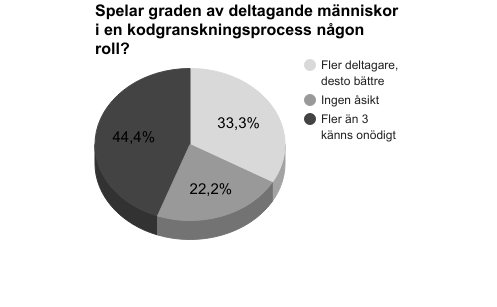
\includegraphics[width=110mm]{figures/grade_participation.png}
	\caption{Resultatet från om antalet deltagande människor i en kodgranskningsprocess spelar någon roll.}
	\label{fig:grade_participation}
\end{figure}

\section{Diskussion}
\label{sec:discussion-wallstrom}
Resultatet av den genomförda enkäten visar att effekterna av en kodgranskningsprocess är positiva. 100 \% av de tillfrågade anser att kodgranskning hjälper till att kvalitetssäkra en produkt. Det är endast få personer som inte använt sig av den specifika metoden kodgranskning för att kvalitetssäkra en produkt, utan istället använt sig av parprogrammering. Datan ifrån enkäten är inte tillräcklig och är en avgränsning i denna studie, för en mer representativ bild skulle det krävas större mängd data. 

Det intressanta med resultatet ifrån enkäten är att 44,4 \% av de som deltog anser att om fler än tre personer deltar i en kodgranskningsprocess finns det risk att tidsåtgången inte kompenserar för den faktiska vinsten med granskningen. Detta är också något som Beller et al. \cite{beller2014modern} kommer fram till i sin studie angående vilka problem som löses med hjälp av kodgranskning. Beller anser att en homogen kodgranskning, det vill säga en likartad kodgranskning beroende på vem som utför den, leder till samma antalet ändringar i koden oberoende av vem som granskar. Det spelar alltså inte någon roll vem som granskar koden, den kommer heller inte blir bättre desto fler som granskar. Resultatet tyder alltså på att en kodgranskningsprocess inte bör innehålla fler deltagande personer än tre för att kvalitetssäkra produkten. 

Samtidigt visar McIntosh et al. \cite{mcintosh2014impact} att kodgranskningsprocesser med lågt deltagande uppskattningsvis innehåller upp till fem stycken defekter, vilket kan låta som en kontradiktion till Beller et al.'s \cite{beller2014modern} resultat. McIntosh specificerar dock inte att det finns ett optimalt antal personer som ska delta i en kodgranskningsprocess för att göra den så effektiv och kvalitetssäkrande som möjligt. Den intressanta fråga som då ställs är om det finns ett optimalt antal deltagande personer i en kodgranskningsprocess? Det är en fråga som utifrån egna slutsatser inte finns något svar på. Det är en bred fråga och beror på hur stort projektet är och vad det finns för kvalitetsmål på produkten. Ju högre kvalitetsmål, desto fler personer bör delta i kodgranskningsprocesserna känns intuitivt som ett bra tillvägagångssätt. Denna studie visar dock att så inte är fallet, kodgranskningen riskerar att bli ineffektiv vilket således kan leda till en icke komplett produkt. Det här är en intressant frågeställning som kräver vidare efterforskning. Även här finns det såklart avgränsningar som bör tas med i åtanke. Dels innehåller inte enkäten tillräckligt med data och därtill skulle det även behövas göra en mer omfattande litteraturstudie för att få en representativ bild över situationen.

\subsection{Källkritik}
Det finns många artiklar som handlar om just kodgranskning och vad denna process har för inverkan på kvalitet. De två artiklar som användes i resultat för denna studie valdes för att de experiment som de genomfört var relevanta för min studie. 

McIntosh et al.'s \cite{mcintosh2014impact} studie har i skrivandets stund citerats av 84 stycken andra publicerade artiklar. McIntosh har även en bred repertoar med publicerade artiklar och flera av dem handlar om just kodgranskning och dess påverkan av kvalitet.

Bellers et al.'s \cite{beller2014modern} studie har i skrivandets stund citerats av 55 stycken publicerade artiklar. Beller har inte heller en lika bred repertoar i publicerade artiklar som McIntosh har, han har däremot flera artiklar som blivit väl citerade som handlar om testning. Som nämnts tidigare är testning en stor del i att kvalitetssäkra en produkt. Jag tycker att Bellers och McIntosh artiklar anses pålitliga och har därför använts i denna studie.

De källor som användes till teorin stämmer inte överens med de källor som representerar studiens resultat. Anledningen till detta är att de artiklar som representar resultat i studien inte presenterar vad kvalitetssäkring och kodgranskning innebär på ett elementärt vis. Detta leder till att resultatet kan tyckas bli mindre trovärdigt. Jag ser det dock som att både McIntosh et al.'s- \cite{mcintosh2014impact} och Bellers et al.'s \cite{beller2014modern} artikel förutsätter att läsaren vet vad kvalitetssäkring och kodgranskning innebär och behöver således inte förklaras mer ingående. På grund av detta har jag valt att använda olika artiklar till teoridelen och resultatdelen.

\section{Slutsatser}
\label{sec:conclusions-wallstrom}
Utifrån den genomförda enkäten men framförallt utifrån den gjorda litteraturstudien visar denna rapport att kvalitet och kodgranskning har en stark relation. Att genomföra en kodgranskningsprocess visar sig tydligt ha positiva effekter på produktens kvalitet. För att svara på fråga 1 i avsnitt \ref{sec:issue-wallstrom} så tyder resultatet från denna studie på att effekterna av en kodgranskningsprocess är positiva ur kvalitetssynpunkt. McIntosh et al. \cite{mcintosh2014impact} visar att en dåligt granskad kod, det vill säga kod som granskats av få personer, kan skapa mellan två till fem stycken defekter.

För att svara på fråga 2 i avsnitt \ref{sec:issue-wallstrom} så tyder resultatet från denna studie att kostnaden för en kodgranskningsprocess kompenserar för den faktiska tidsåtgången. Den genomförda enkäten visade att 100 \% av deltagarna anser att kodgranskning hjälper till att kvalitetssäkra en produkt. Enkäten visar också att antalet deltagande människor i kodgranskningen inte behöver överstiga tre stycken, detta kan leda till onödig tidsåtgång. Det här är även något som bekräftas av Bellers et al.'s \cite{beller2014modern} studie. Slutsatsen av detta är att effekterna av en kodgranskningsprocess kompenserar den faktiska tidsåtgången så länge antalet personer som granskar inte överstiger tre stycken.


%%%%%%%%%%%%%%%%%%%%%%%%%%%%%%%%%%%%%%%%%%%%%%%%%%%%%%%%%%%%%%%%%%%%%%
%%% person-report.tex ends here
